\documentclass[journal]{IEEEtran}

\usepackage{amscd,amssymb}
\usepackage{amsfonts}
\usepackage{url}
\usepackage{xspace}
%\usepackage[pdfusetitle,colorlinks,plainpages=false]{hyperref}
%\usepackage{biblatex}
\usepackage{tikz}
\usepackage{tikz-qtree}
\usepackage{tikz-uml}
\usepackage[caption=false]{subfig}
\usepackage{tabularx}
\usepackage{color}
\usepackage{amsmath}
\usepackage{listings}
\usepackage{units}
%\usepackage{amsthm}
\usepackage{algpseudocode}
\usepackage{algorithm}
% \usepackage[T1]{fontenc} \usepackage{lmodern}

\newenvironment{keywords}{
       \list{}{\advance\topsep by0.35cm\relax\small
       \leftmargin=0cm
       \labelwidth=0cm
       \listparindent=0cm
       \itemindent
       \listparindent
       \rightmargin\leftmargin
       }
  \item[\hskip\labelsep
                                     \bfseries Keywords:]}
     {\endlist}

%\theoremstyle{definition}
\newtheorem{defn}{Definition}
\newtheorem{thm}{Theorem}
\newtheorem{corr}{Corollary}

\definecolor{dkgreen}{rgb}{0,0.6,0}
\definecolor{gray}{rgb}{0.5,0.5,0.5}
\definecolor{mauve}{rgb}{0.58,0,0.82}

\lstdefinelanguage{PIL}{
morekeywords={ExecutionOrder, Common, Prover, Verifier, Def, Void, Prime, Z, Int},
otherkeywords={Zmod+, Zmod*},
morecomment=[l]{//},
morecomment=[s]{/*}{*/}
}

\lstdefinelanguage{PSL}{
  morekeywords={Prime, Public, ProverPrivate,
    KnowledgeError, SZKParameter, ProtocolComposition, Homomorphism,
    ChallengeLength, SigmaPhi, Relation, Declarations, Inputs, Properties},
  otherkeywords={Zmod+, Zmod*},
  morecomment=[l]{//}, morecomment=[s]{/*}{*/}
}

\lstdefinelanguage{grammar}{
  keywords={},
  otherkeywords={}
}

\lstdefinelanguage{GEZEL}{
  morekeywords={sfg, dp, always, reg, syg, system, ns, tc, out, in, use, sig},
  otherkeywords={$display, $hex, $dec, $bin, $cycle},
  morecomment=[l]{//}
}

\lstset{
language=PIL,
basicstyle=\footnotesize,
commentstyle=\color{dkgreen},
keywordstyle=\bfseries,
frame=single,
breaklines=true,
breakatwhitespace=false
}

\usetikzlibrary{backgrounds,calc,shapes,shapes.geometric,shadows,arrows,chains,trees,fit,positioning}

\tikzstyle{language}=[rectangle,draw=black,thin,inner sep=3pt, align=center]

\tikzstyle{compiler}=[rectangle,rounded corners,draw=black,thin,inner
sep=3pt, align=center]

\tikzstyle{added}=[fill=gray]

\begin{document}

\title{Implementation and Evaluation of Zero-Knowledge Proofs of Knowledge}

\author{
Boran Car, Josep Balasch, Alfredo Rial, Ingrid Verbauwhede and Bart Preneel}

\maketitle

\begin{abstract}
  Zero-Knowledge Proofs of Knowledge allow one to prove possession or
  knowing of a certificate without actually revealing the secret. This
  involves using a hard problem as a basis for the protocol. Goals of
  current Zero-Knowledge Proofs of Knowledge compiler frameworks are
  to make this process easy for those outside the field of
  cryptography while at the same time making it easy for those inside
  the field to develop such protocols.

  We acknowledge that such frameworks have made it easy to develop the
  protocols but we note that they have not made it easy or general to
  those implementing the protocols on the end devices. Such frameworks
  either target C code generation or an interpreted language. They
  also use high-level multi-precision arithmetic libraries which are
  too resource hungry for small embedded devices. These limitations
  have motivated us to extend one of those frameworks and build our
  own framework from it. This framework is targeted specifically at
  small embedded devices while not losing any generality of the
  framework it extends.

\begin{keywords}
  zero-knowledge, proofs of knowledge, 
\end{keywords}

\end{abstract}

%%% Local Variables: 
%%% TeX-PDF-mode: t
%%% TeX-master: "main"
%%% End: 


\section{Introduction}
\label{introduction}
%1.1-	Motivation
%- Crypto involves complex building blocks.
%- Among them, ZKPK.
%- Its implementation is complex
%- most programmers are not cryptographers, and thus prone to errors
%- Automated tools for implementing crypto protocols are needed (name some existing tools).
%
%- crypto implementations for embedded devices are demanded
%- new crypto protocols
%- generic tools (GMP, high java level)
%- Existing tools should be adapted to embedded devices.

%In the last years myriad of advanced cryptographic techniques have been proposed and formalized in the open literature. Such protocols go beyond the traditional security goals of data integrity, authentication, and confidentiality, and instead focus on providing other strong security and privacy properties.
%
%Zero-knowledge proofs of knowledge~\cite{Goldwasser:1985:KCI:22145.22178,Goldreich:1987:PNZ:36664.36675,springerlink:10.1007/BF02351717} are amongst the most prominent examples of this trend. These cryptographic tools allow an entity (the \emph{Prover}) to prove knowledge of a statement to another entity (the \emph{Verifier}) without actually revealing any information about such statement. Within a system, ZKPoK can be used to enforce honest behaviour between entities while maintaining their privacy, making such protocols ideal for privacy preserving applications. Just to name a few, zero-knowledge proofs of knowledge are found at the core of systems such as anonymous e-cash~\cite{1982-1101,Camenisch05compacte-cash}, anonymous authentication~\cite{Brickell:2004:DAA:1030083.1030103,Nguyen05dynamick-times}, or electronic voting~\cite{Groth:2005:NZA:2134532.2134564,Damgard03thetheory}.

Zero-knowledge proofs of knowledge (ZKPK)~\cite{Goldwasser:1985:KCI:22145.22178,Goldreich:1987:PNZ:36664.36675,springerlink:10.1007/BF02351717} allow an entity (the \emph{Prover}) to prove knowledge of a secret that fulfills a statement to another entity (the \emph{Verifier}) without revealing any information about the secret. ZKPK can be used as building blocks of cryptographic protocols to enforce the honest behaviour of entities while maintaining their privacy, making such protocols ideal for privacy preserving applications. Just to name a few, ZKPK are found at the core of systems such as anonymous e-cash~\cite{DBLP:conf/crypto/Chaum82,Camenisch05compacte-cash}, anonymous authentication~\cite{Brickell:2004:DAA:1030083.1030103,Nguyen05dynamick-times}, electronic voting~\cite{Groth:2005:NZA:2134532.2134564,Damgard03thetheory} or general secure two-party and multi-party computation~\cite{DBLP:conf/stoc/CanettiLOS02}.

%Such strong security properties come however at a high cost in terms of complexity and efficiency. 

The implementation of ZKPK is error-prone, particularly for programmers not familiar with the underlying cryptographic techniques, which hinders the deployment of protocols that employ ZKPK. To address this problem, there exist nowadays several tools to facilitate ZKPK implementation, either by providing high-level libraries~\cite{Camenisch:2002:DII:586110.586114}, custom made language interpreters and compilers~\cite{Almeida:2010:CCZ:1888881.1888894}, or a mixture of both~\cite{Meiklejohn:2010:ZLS:1929820.1929838}.

Existing tools~\cite{Camenisch:2002:DII:586110.586114,Almeida:2010:CCZ:1888881.1888894,Meiklejohn:2010:ZLS:1929820.1929838} target software (SW) high-level languages such as C, C++ or Java. However, some protocols are naturally expected to be implemented on small embedded platforms, e.g.\ smart cards for storing e-cash wallets, and electronic IDs or TPMs for anonymous authentication~\cite{Brickell:2004:DAA:1030083.1030103}. In such cases, the use of ZKPK compilers that target hardware (HW) description languages and that allow for HW-SW co-design is more convenient.

%While incredibly useful, these tools focus on ZKPoKs as standalone blocks rather than as part of a full application. In other words, there are some limitations such as e.g.\ when implementing systems with multiple participating entities. Similarly, the resulting code is given in high-level languages such as C, C++, or Java, each one using their own cryptographic library, making it difficult to port the code to small embedded devices. This is of importance since, as can be noted from the above mentioned examples, some entities are naturally expected to be implemented on small embedded platforms, e.g.\ smart cards for storing e-cash wallets, electronic IDs or TPMs for anonymous authentication, etc...

%1.2- Our contribution
%- We do not start from scratch
%- We use an existing framework, which we extend and modify
%- Explanation on the main extensions and modifications (why the extension/modification was needed, which functionalities are now possible that were not possible before).
%- Explanation of the new features provided. Focus on all the implementation possibilities (HW languages, embedded devices, HW-SW codesign).
\paragraph{Our contribution.} We provide a ZKPK compiler framework specifically tailored to target hardware description languages and HW-SW co-design. Rather than starting from scratch, we extend the functionalities offered by the CACE ZKPK compiler suite~\cite{Almeida:2010:CCZ:1888881.1888894} to generate platform-independent code and explore hardware/software boundaries. The CACE ZKPK compiler allows the implementation of (the composition of) the most relevant $\Sigma$-protocols, which are the practically relevant ZKPK. 

Concretely, our ZKPK compiler framework follows two steps. First, it takes as input a ZKPK implementation in platform-independent code generated by the CACE ZKPK compiler and transforms it into an implementation in LLVM IR, which is the intermediate representation language of the LLVM compiler framework. The implementation in LLVM IR can be optimized via the LLVM optimizer.

From LLVM IR, it is possible to target different languages. We provide a back-end for GEZEL, a HW description language that can subsequently target VHDL or Verilog, that provides validation tools and that offers a co-simulation tool used for HW-SW co-design purposes. Additionally, we provide a back-end for C, which uses GMP for big integer arithmetic. Therefore, we cover both ends of the HW/SW co-design spectrum.

We consider that our custom ZKPK compiler framework provides a good starting point for a fine-grained automated approach to HW-SW co-design. It  allows the implementation of all the ZKPK supported by the original CACE ZKPK compiler. Additionally, thanks to the characteristics of LLVM IR, we can validate the security of the implementation at a lower level than the one allowed by the CACE ZKPK compiler.

%1.3- Structure of the paper (Explain briefly the contents of each section of the paper)
\paragraph{Structure of the paper.} In Section~\ref{relatedwork} we summarize related work in the area of cryptography aware compilers. In Section~\ref{preliminaries} we provide some background information. The tools used through the paper are briefly introduced in Section~\ref{sec:tools}. Our custom compiler is described in Section~\ref{customframework}, and some discussion topics are addressed in Section~\ref{discussion}. Finally we conclude in Section~\ref{conclusion}.

%%% Local Variables:
%%% TeX-PDF-mode: t
%%% TeX-master: "paper"
%%% End:


\section{Related Work}
\label{relatedwork}

The need for cryptographically aware compilers is extensively motivated by Bangerter et al.~\cite{citeulike:7079130}. A number of compiler based tools have been proposed recently. Some target a wide variety of cryptographic primitives and protocols~\cite{DBLP:conf/weworc/LucksST05,DBLP:conf/issa/BangerterKSU11}, while others focus on specific areas, such as multiparty computation~\cite{DBLP:conf/uss/MalkhiNPS04,DBLP:conf/pkc/DamgardGKN09,DBLP:conf/ccs/HeneckaKSSW10} and ZKPK.

A first example of ZKPK compiler was proposed in~\cite{TUD-CS-2005-0034} and extended in \cite{DBLP:conf/europki/BangerterBHKSS09}. Subsequently, Almeida et al. proposed the CACE ZKPK compiler~\cite{CACE}, which allows the implementation of most relevant $\Sigma$-protocols. The CACE ZKPK compiler avoids security vulnerabilities by choosing certain security parameters automatically and by validating the implementations via a formal theorem prover. A more detailed description is given in Section~\ref{sec:tools}.

Another ZKPK compiler (ZKPDL) was proposed by Meiklejohn et al.~\cite{Meiklejohn:2010:ZLS:1929820.1929838}. When compared to CACE, ZKPDL improves efficiency by using precomputation, but allows the implementation of a narrower class of protocols and does not provide formal verification. A detailed comparison between CACE and ZKPDL is given in \cite{Bangerter_yaczk:yet}.

To the best of our knowledge, currently there is no compiler that targets HW specification languages or that allows for HW-SW co-design.

 



%-	ZKPDL
%-	Other related work (take from the paper “A Certifying Compiler for Zero-Knowledge Proofs of Knowledge Based on Sigma-Protocols”

%%% Local Variables:
%%% TeX-PDF-mode: t
%%% TeX-master: "main"
%%% End:


\section{Background}
In this section we review necessary background information. In the
first part, we describe the targeted ZKPK $\Sigma$-protocols and in
the second part, we provide definitions of data flow graph and
control flow graph.
\label{preliminaries}
\chapter{Technical Preliminaries}

This chapter has the goal of introducing the math and theory behind
formal languages, parsers, algebra, (zero knowledge) proofs of
knowledge, control and data flow in a program. Knowledge behind formal
languages is needed to design a parser which will later on be used to
create a custom compiler framework.

Zero knowledge proofs of knowledge are the basis of this thesis so
they need to be introduced here. First we start with group theory and
modular arithmetic, then we proceed with defining zero knowledge proofs
of knowledge and give a basic example of a protocol.

We conclude the chapter with introducing control flow graphs and data
flow (data dependency) graphs which are needed to reason about the
intermediate form the compiler generates.

\section{Formal Languages}

The theory of formal languages is needed to introduce a parser which
is the basic building block of a compiler. Here we give a short
overview of formal languages based on \cite{formal_languages} and for
a more detailed approach refer the reader to \cite{Hopcroft}.

We start with basic definitions of a formal language:

\begin{defn}[Alphabet]
  An alphabet $\Sigma$ is a set of symbols.
\end{defn}

\begin{defn}[String]
  A string over an alphabet $\Sigma$ is a sequence of symbols of $\Sigma$.
\end{defn}

\begin{defn}[Concatenation]
  Let $x = a_0 a_1 \dotsm a_n$ and $y = b_0 b_1 \dotsm b_n$, then the
  string $x y = a_0 a_1 \dotsm a_n b_0 b_1 \dotsm b_n$ is the
  concatenation of the strings $x$ and $y$.
\end{defn}

\begin{defn}[Sets]
  $\Sigma^*$ denotes the set of all the strings over the alphabet
  $\Sigma$. Likewise, $\Sigma^+$ denotes the set of all the non-empty
  strings over the alphabet $\Sigma$. $$\Sigma^+ \subseteq \Sigma^*
  \setminus \{ \epsilon \}$$ The empty set of strings is denoted
  $\emptyset$.
\end{defn}

\begin{defn}[Language]
  A language over the alphabet $\Sigma$ is a set of strings over
  $\Sigma$. Members of the language are called words of the language.
\end{defn}

\begin{defn}[Concatenation]
  Let $L_1$ and $L_2$ be two languages over alphabet $\Sigma$, the
  language $L_1 L_2 = \{x y | x \in L_1, y \in L_2 \}$ is the
  concatenation of $L_1$ and $L_2$.
\end{defn}

\begin{defn}[Kleene closure]
  Let $L$ be a language over $\Sigma$. Define 
  $$L^0 = \{ \epsilon \}$$
  $$L^i = L L^{i-1} \; \textrm{for} \; i \ge 1$$
  The \emph{Kleene closure} of $L$, denoted by $L^*$, is the language:
  $$ L^* = \bigcup_{i \ge 0} L^i $$
  the \emph{positive closure} is
  $$ L^+ = \bigcup_{i \ge 1} L^i $$
  It can be observed that
  $$ L^* = L^+ \cup \{ \epsilon \} $$
  $$ L^+ = L L^* $$
\end{defn}

We now have a formal basis to define a more powerful tool called
regular expressions. These regular expressions will allow us to
formally, yet compactly, specify the words of a language.

\subsection{Regular Expression}

When writing lexer rules for our compiler, we will need a language
that defines words of the language of our interest. Such a language is
called regular expressions and we briefly define it here:

\begin{defn}[Regular expression]
  A regular expression over $\Sigma$ is defined inductively as follows:
  \begin{enumerate}
  \item $\emptyset$ is a regular expression and represents the empty language
  \item $\epsilon$ is a regular expression and represents the language
    $L = \{ \epsilon \}$
  \item For each $c \in \Sigma$, $c$ is a regular expression and
    represents the language $L = \{ c \}$
  \item For any regular expressions $r$ of language $R$ and $s$ of language $S$:
    \begin{itemize}
    \item $r+s$ is a regular expression representing language $R \cup S$
    \item $r s$ is a regular expression representing language $R S$
    \item $r^*$ is a regular expression representing language $R^*$
    \item $r^+$ is a regular expression representing language $R^+$
    \end{itemize}
  \end{enumerate}
\end{defn}

\begin{thm}
  $r r^*$ can be represented as $r+$
\end{thm}

\begin{proof}
  $r r^*$ represents the language $R R^*$ which is $R^+$
\end{proof}

Now that we have the tool to specify the words of our language, we
need to specify the interactions between these words (e.g. which words
can follow a certain word, what the word ordering is). Such rules are
specified by grammars.

\subsection{Grammars}

When writing parser rules, we will need a language to specify the
interactions between the words of our language. Such a language
is called a grammar and we briefly define it here:

\begin{defn}[Grammar]
  A grammar is a 4-tuple $G = \left< \Sigma, V, S, P \right>$:
  \begin{enumerate}
  \item $\Sigma$ is a finite non-empty set called the \emph{terminal
    alphabet}. The elements of $\Sigma$ are called \emph{terminals}.
  \item $V$ is a finite non-empty set disjoint from $\Sigma$. The
    elements of $V$ are called \emph{non-terminals} or \emph{variables}.
  \item $S \in V$ is a distinguished symbol called the \emph{start symbol}
  \item $P$ is a finite set of \emph{productions (rules)} of the form
    $$ \alpha \rightarrow \beta $$
    $$ \alpha \in (\Sigma \cup V)^* V (\Sigma \cup V)^* $$
    $$ \beta \in (\Sigma \cup V)^* $$
  \end{enumerate}
\end{defn}

\begin{defn}[Context-free grammar]
  The grammar $G$ is a context free grammar iff $|\alpha|$ = 1 ($\alpha = V$).
\end{defn}

We now have all the tools to specify the input language of our
compiler. The parser of our compiler will transform an input file,
according to these rules, to a form suitable for further
processing. The forms we deal at this step are concrete syntax trees
and abstract syntax trees.

\subsection{Concrete Syntax Tree}

A Concrete Syntax Tree, also called a Parse Tree, is an ordered tree
representation of the input according to a given formal grammar.

For example, given the following input:
\begin{lstlisting}
a := b * c + d;
\end{lstlisting}
and the following grammar:
\begin{align*}
  \textrm{statement}  & \rightarrow \textrm{ID} := \textrm{expression} ; \\
  \textrm{expression} & \rightarrow \textrm{term} + \textrm{term} \\
  \textrm{term}       & \rightarrow \textrm{ID} * \textrm{ID} \\
  \textrm{term}       & \rightarrow \textrm{ID}
\end{align*}
the tree depicted in Figure \ref{fig:simple_cst} is a Concrete Syntax Tree.

\begin{figure}[hbt!]
  \centering
  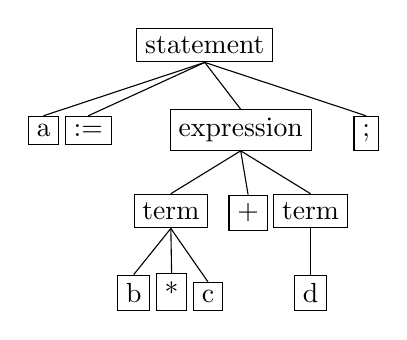
\begin{tikzpicture}
    \Tree [.\node[language](statement){statement};
      [.\node[language](a){a};]
      [.\node[language](assign){:=};]
      [.\node[language](expression){expression};
        [.\node[language](term){term};
          [.\node[language](b){b};]
          [.\node[language](mul){*}; ]
          [.\node[language](c){c};]
        ]
        [.\node[language](plus){+};]
        [.\node[language](term2){term};
          [.\node[language](d){d};]
        ]
      ]
      [.\node[language](semi){;};]
    ]
  \end{tikzpicture}
  \caption{Concrete Syntax tree for a simple input and a simple grammar}
  \label{fig:simple_cst}
\end{figure}

\subsection{Abstract Syntax Tree}

An Abstract Syntax Tree (AST) is a tree representation of the abstract
syntax of the input. Given the same example
\begin{lstlisting}
a := b * c + d;
\end{lstlisting}
one possible variant of the tree is illustrated in Figure
\ref{fig:simple_ast}. Comparing it with the Parse Tree from Figure
\ref{fig:simple_cst} one can see that the choice of abstraction is
arbitrary.

\begin{figure}[hbt!]
  \centering
  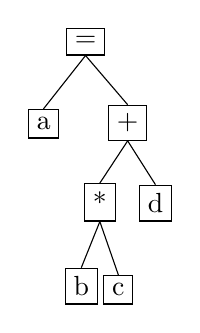
\begin{tikzpicture}
    \Tree [.\node[language](equ){=};
      [.\node[language](a){a};]
      [.\node[language](add){+};
        [.\node[language](mul){*};
          [.\node[language](b){b};]
          [.\node[language](c){c};]
        ]
        [.\node[language](d){d};]
      ]
    ]
  \end{tikzpicture}
  \caption{An example AST for a simple expression}
  \label{fig:simple_ast}
\end{figure}

After all the definitions of the input and the output have been made,
it remains to define the actual tool transforming from the input to
the output. This tool is referred to as the parser.

\subsection{Parser}

Given a string $L$, satisfying grammar $G$, a parser tries to find the
derivation of $L$ from $S$. This derivation is the Concrete Syntax
Tree (Parse Tree). This derivation may further be abstracted into an
Abstract Syntax Tree that is easier for later manipulation. Figure
\ref{fig:parser_flow} shows the typical parser flow.

\begin{figure}[hbt!]
  \centering
  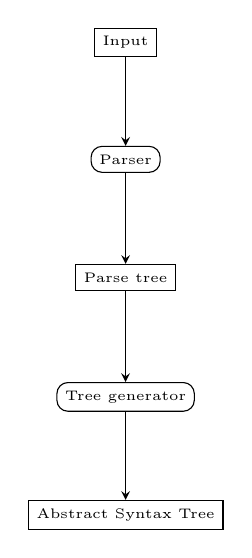
\begin{tikzpicture}[>=stealth,level distance=1.5cm,font=\tiny]
    \tikzstyle{edge from parent}=[draw,->]

    \Tree [.\node[language](input){Input};
      [.\node[compiler](parser){Parser};
        [.\node[language](ptree){Parse tree};
          [.\node[compiler](tgen){Tree generator};
            [.\node[language](ast){Abstract Syntax Tree};
            ]
          ]
        ]
      ]
    ]
  \end{tikzpicture}
  \caption{Parser flow}
  \label{fig:parser_flow}
\end{figure}

There are two approaches to parsing:
\begin{description}
\item[Top-down parsing] the derivation starts from the top (the root)
  of the parse tree and proceeds downwards.
\item[Bottom-up parsing] the derivation starts from the bottom (the
  leaves) of the parse tree and proceeds upwards.
\end{description}

The most popular top-down parser is an LL (left to right left-most
derivation) parser. The parser reads the input left to right and at
each step produces the left-most derivation of the input. Sub-types of
this parser include the symbol look-ahead which is the amount of next,
unseen symbols the parser can ``look at''. For example, an LL(1)
parser can only look 1 symbol ahead while an LL(*) parser is a parser
with arbitrary look-ahead.

\section{Group Theory and Modular Arithmetic}

Before we go into defining proofs of knowledge we need to define the
space we are operating on. We base our definitions on \cite{HAC}, but
the approach we take is a bit different. We choose to start with the
general and deduce the specific from it rather than taking an
inductive approach.

\begin{defn}[Group]
  A group $(G, \circ)$ is a set G with a binary operation $\circ$ defined on it
  that satisfies the following properties:
  \begin{enumerate}
  \item (Closure) $a, b \in G \implies a \circ b \in G$ 
  \item (Associativity) $(a \circ b) \circ c = a \circ (b \circ c)$ $\forall a,b,c \in G$
  \item (Identity element) $\exists I \in G$ such that $a \circ I = I \circ a = a$
  \item (Inverse element) ($\forall a \in G)(\exists a^{-1} \in G)$ such that $a \circ
    a^{-1} = a^{-1} \circ a = I$
  \end{enumerate}
\end{defn}

\begin{defn}[Abelian Group]
  A group $G$ is abelian iff $a \circ b = b \circ a$ $\forall a,b \in G$
\end{defn}

\begin{defn}[Finiteness and Order]
  A group $G$ is finite iff $|G|$ is finite. The number of elements in
  $G$ is called the \emph{order} of the group.
\end{defn}

\begin{defn}[Subgroup]
  A non-empty subset $H \subseteq G$ is a subgroup iff $H$ itself is a
  group w.r.t. to the binary operation of $G$. $H$ is a proper subgroup
  iff $H \neq G$.
\end{defn}

\begin{defn}[Cyclic Group]
  A group $G$ is cyclic iff $(\exists a \in G)(\forall b \in G)(i is
  Integer | b = a^i)$. Such an $a$ is called a generator of $G$. The
  group generated by $a$ is denoted as $\left< a \right>$.
\end{defn}

\begin{defn}[Order]
  Let $G$ be a group and $a \in G$. The order of $a$ is the least
  positive integer $t$ such that $a^t = I$, provided that such an
  integer exists.  If such an integer does not exist, the order is
  defined to be $\infty$.
\end{defn}

\begin{thm}[Lagrange's Theorem]
  If $G$ is a finite group and $H$ is a subgroup of $G$ then $|H|$ divides
  $|G|$.
\end{thm}

\begin{corr}
  The order of $a \in G$ divides $|G|$.
\end{corr}

\begin{defn}[Congruency]
  An integer $a$ is said to be congruent to integer $b$ modulo integer
  $n$, written $a \equiv b \pmod{n}$, iff $n$ divides $a-b$ (denoted as
  $n | a - b$). $n$ is called the \emph{modulus} of the congruency.
\end{defn}

\begin{defn}[Greatest Common Divisor]
  Given two integers $a$ and $b$, the greatest common divisor
  $d=\gcd(a,b)$ is the largest integer $d$ such that $d | a$ and $d | b$.
\end{defn}

\begin{defn}
  Two integers, $a$ and $b$, are relatively prime to each other iff
  \mbox{$\gcd(a,b)=1$}.
\end{defn}

\begin{defn}
  The integers modulo $n$, denoted $Z_n$, is the set of integers
  \mbox{$\{ 0,1,2,\ldots,n-1 \}$}.
\end{defn}

\begin{thm}
  Let $d = \gcd(a, n)$. Then the congruence equation $a x = b \pmod{n}$ has
  $d$ solutions $x$ iff $d$ divides $b$.
\end{thm}

\begin{corr}
  Let $a \in Z_n$. $a$ has a multiplicative inverse, denoted $a^{-1}$,
  iff \mbox{$\gcd(a, n) = 1$}.
\end{corr}

\begin{defn}
  The multiplicative group of $Z_n$ is $Z_n^* = \{a | \gcd(a,n) = 1
  \}$.  Specifically, if $n$ is prime, $Z_n^* = \{a | 1 \leq a \leq n-1
  \}$. The identity element of the multiplicative group is $1$.
\end{defn}

\begin{defn}
  The additive group of $Z_n$ is $Z_n^+ = \{a | 0 \leq a \leq n-1 \}$.
\end{defn}

\begin{defn}[Euler Phi Function]
  The Euler phi function, $\phi(n)$, also called Euler totient
  function, gives the number of integers from the interval $[1,n]$
  which are relatively prime to $n$.
\end{defn}

\begin{corr}
  The order of the group $Z_n^*$ is $\phi(n)$.
\end{corr}

\begin{corr}
  For a prime $p$, $\phi(p) = p-1$.
\end{corr}

\begin{corr}
  If $\gcd(m, n) = 1$, $\phi(m n) = \phi(m) \phi(n)$.
\end{corr}

\begin{thm}[Euler's Theorem]
  If $a \in Z_n^*$, then $a^{\phi(n)} = 1 \pmod{n}$.
\end{thm}

\begin{corr}[Fermat's Theorem]
  If $a \in Z_p^*$, where $p$ is prime, then $a^{p-1} = 1 \pmod{p}$.  
\end{corr}

\begin{corr}
  $a \in Z_n^*$ is a generator of the group $Z_n^*$ iff the order of
  $a$ is $\phi(n)$. $a$ is also called a primitive element of $Z_n^*$
  then.
\end{corr}

After defining the space we are operating on, it remains to define the
basis of this thesis, zero knowledge proofs of knowledge.

\section{Zero Knowledge Proofs of Knowledge}

Zero knowledge proofs of knowledge give us a powerful tool that allows
us to prove knowledge of a secret without actually revealing the
secret.  Here we need a more formal definition which we take from
\cite{Cameni98} and present as a brief overview. Some minor additions
were added for clarity.

\begin{defn}[Interactive Proof of Knowledge]
  Let $R \subseteq \{0,1\}^* \times \{0,1\}^*$ be a polinomially
  bounded binary relation and let $L_R$ be the language defined by
  $R$. An interactive proof of knowledge is a protocol $(P, V)$ that
  has the following properties:
  \begin{enumerate}
  \item (Completeness) $(x,w) \in R \implies [V, P(w)](x) = T$
  \item (Validity) There exists a probabilistic expected polynomial-time
    machine $K$ (Knowledge extractor) such that for every $\tilde{P}$, for
    all polynomials $f(\cdot)$ and all sufficiently large $x \in L_R$:
    \[
    p((x, K^{\tilde{P}(x)}) \in R) \geq p([V, \tilde{P}](x) = T) -
    \frac{1}{f(|x|)}
    \]
    The probabilities are taken over all random choices of $V$, $P$,
    $\tilde{P}$, $K$. The notation $\left[V, P(w)\right](x)$ denotes
    the protocol execution with the secret $x$ and the prover output
    $w$. $\tilde{P}$ includes malicious provers. $K^{\tilde{P}(x)}$
    denotes oracle access to $\tilde{P}(x)$. $f(\cdot)$ denotes the
    knowledge error.
  \end{enumerate}
\end{defn}

\begin{defn}[Soundness] $(\forall \tilde{P})(\forall x \notin
  L_R)(p([V, \tilde{P}](x) = T) < \frac{1}{2})$
\end{defn}
The additional soundness property is associated with $x \notin L_R$.  By
repeating the protocol many times, it can be made arbitrarily small
\cite{Cameni98}.

\begin{defn}[Indistinguishability]
  Let $L \in \{0,1\}^*$ be a language and let $A = \{A(x)\}_{x \in L}$
  and $B = \{B(x)\}_{x \in L}$ be two ensembles of random variables
  indexed by $L$. Ensembles $A$ and $B$ are:
  \begin{itemize}
  \item perfectly indistinguishable if for all $x \in L$ the variables
    $A(x)$ and $B(x)$ are identically distributed
  \item statistically indistinguishable if for every polynomial $f()$
    and for all sufficiently long $x \in L$:
    \[
    \sum_{\alpha \in \{0,1\}^*} | p(A(x) = \alpha) - p(B(x) = \alpha)|
    < \frac{1}{f(|x|)}
    \]
  \item computationally indistinguishable if for every probabilistic
    polynomial-time algorithm $D$, for every polynomial $f()$ and for
    all sufficiently long $x \in L$:
    \[
    |p(D(x, A(x) = 1) - p(D(x, B(x) = 1)| < \frac{1}{f(|x|)}
    \]
  \end{itemize}
\end{defn}

\begin{defn}[Zero-Knowledge]
  An interactive protocol $(P, V)$ is said to be
  perfectly/statistically/computationally zero-knowledge if for
  every probabilistic polynomial-time verifier $\tilde{V}$ there
  exists a probabilistic expected polynomial time simulator
  $S_{\tilde{V}}$ so that the two ensembles
  \[
  \{[\tilde{V}, P(w)](x)\}_{x \in L} \; \textrm{and} \; \{S_{\tilde{V}}(x)\}
  \]
  are perfectly/statistically/computationally indistinguishable.
\end{defn}

\begin{defn}[Honest Verifier Zero-Knowledge]
  An interactive protocol $(P, V)$ is said to be
  perfectly/statistically/computationally zero-knowledge if there
  exists a probabilistic expected polynomial time simulator
  $S_{\tilde{V}}$ so that the two ensembles
  \[
  \{[V, P(w)](x)\}_{x \in L} \; \textrm{and} \; \{S_V(x)\}
  \]
  are perfectly/statistically/computationally indistinguishable.
\end{defn}

To make a more practical definition we restrict to a subset of zero
knowledge proofs of knowledge called $\Sigma$-protocols.

\subsection{$\Sigma$-protocols}

A $\Sigma$-protocol is a three round honest verifier zero-knowledge
proof of knowledge \cite{cryptography_introduction}. The name comes
from the protocol's flow resemblance to the Greek letter $\Sigma$ as
shown in Figure \ref{fig:sigma_flow}. The rounds of the protocol are:
\begin{enumerate}
\item Commitment ($t$) - the prover commits to a value and sends that
  value to the verifier
\item Challenge ($c$) - the verifier computes a random challenge and asks
  the prover to output a value for that challenge
\item Response ($s$) - the prover responds with a new computed value
\end{enumerate}

\begin{figure}[h]
  \centering
  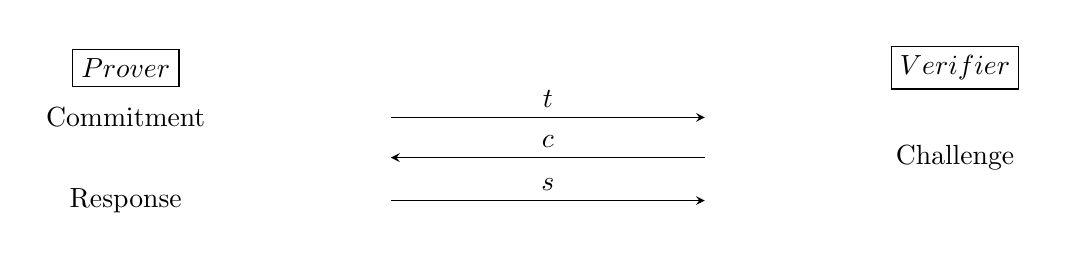
\begin{tikzpicture}[>=stealth]
    \node[matrix,column sep=2cm] {
      \node{\boxed{Prover}};                  &                           & &                             & \node{\boxed{Verifier}}; \\
      \node{Commitment};          & \node(commitment_s){}; & & \node(commitment_r){}; & \\
                                      & \node(challenge_r){}; & & \node(challenge_s){}; & \node{Challenge}; \\
      \node{Response}; & \node(response_s){}; & & \node(response_r){}; & \\
    };
    \draw[->] (commitment_s) -- (commitment_r) node[midway, anchor=south]{$t$};
    \draw[<-] (challenge_r) -- (challenge_s) node[midway, anchor=south]{$c$};
    \draw[->] (response_s) -- (response_r) node[midway, anchor=south]{$s$};
  \end{tikzpicture}
  \caption{Sigma protocol flow}
  \label{fig:sigma_flow}
\end{figure}

\subsubsection{Schnorr's Identification Protocol}
\label{subsubsec:schnorr_protocol}

A simple example of a $\Sigma$ protocol is Schnorr's Identification
Protocol \cite{schnorr_protocol, cryptography_introduction}. The
secret is a discrete logarithm $x$ of $y$ with respect to $g$ in some
finite group $G = \left< g \right>$ with prime order $q$, subgroup of
$Z_p^*$. The prover must prove knowledge of this secret to a verifier
under the homomorphism $f(a) : Z_q^+ \rightarrow G \subset Z_p^* :=
g^a$. Figure \ref{fig:schnorr_steps} gives an overview of the protocol
execution.

\begin{figure}[h]
  \centering
  \begin{tikzpicture}[>=stealth]
    \node[matrix,column sep=2cm] {
      \node{\boxed{Prover}};                  &                           & &                             & \node{\boxed{Verifier}}; \\
      \node{$r_1 \in Z_q^+$};                   &                           & &                             &                   \\
      \node{$t_1 = g^{r_1}$};          & \node(prover_round1_s){}; & & \node(verifier_round1_r){}; & \\
                                      & \node(prover_round2_r){}; & & \node(verifier_round1_s){}; & \node{$c \in \{0,1\}^*$}; \\
      \node{$s_1 = r_1 + x \cdot c$}; & \node(prover_round2_s){}; & & \node(verifier_round2_r){}; & \\
                                      &                           & &                             & \node{$s_1 \stackrel{?}{\in} Z_q^+$}; \\
                                      &                           & &                             & \node{$t_1 y^c \stackrel{?}{=} g^{s_1}$}; \\
    };
    \draw[->] (prover_round1_s) -- (verifier_round1_r) node[midway, anchor=south]{$t_1$};
    \draw[<-] (prover_round2_r) -- (verifier_round1_s) node[midway, anchor=south]{$c$};
    \draw[->] (prover_round2_s) -- (verifier_round2_r) node[midway, anchor=south]{$s_1$};
  \end{tikzpicture}
  \caption{Schnorr's Identification Protocol}
  \label{fig:schnorr_steps}
\end{figure}

\subsubsection{Camenisch-Stadler Notation}
\label{subsubsec:camenisch_stadler}

A simple and popular notation for specifying Sigma protocols is the
Camenisch-Stadler notation \cite{camenisch_stadler}. The Schnorr
Identification Protocol can be represented by the following:
\[
  \textrm{ZPK}\left[ (x): y = g^x \right]
\]
meaning prove knowledge of $x$, using a zero knowledge proof of
knowledge, such that $y=g^x$.

\filbreak

\section{Data Flow Graph and Control Flow Graph}

Our compiler will generate an intermediate form used for detailed
processing. This form is supposed to represent all the operations of
the protocol and can be represented as a directed graph detailing the
flow of the program.

The protocol is input via a text-file and is inherently
sequential. This means that the operations are laid out one after the
other. This inherently imposed ordering need not be the only one and
to make a better ordering w.r.t. to some goal we need constructs that
will allow us to extract all the constraints on the ordering. We keep
the nodes representing the operations while we classify each of the
edges as either a Data Edge or a Control Edge:
\begin{defn}[Data Edge]
  A data edge is an ordered relation between two operations such that
  the output/result of one operation is the input to the other.
\end{defn}
\begin{defn}[Control Edge]
  A control edge is an ordered relation between two operations such
  that the second operation has to be executed after the first finishes
  executing.
\end{defn}

The resulting graph can be separated into two independent graphs called
a Data Flow Graph and a Control Flow Graph.

\begin{defn}[Data Flow Graph]
  A data flow graph is a graph of the nodes representing the
  operations connected by data edges.
\end{defn}

\begin{defn}
  A control flow graph is a graph of the nodes representing the
  operations connected by control edges.
\end{defn}

A Data Flow Graph (DFG) completely and uniquely specifies the
algorithm, whereas the Control Flow Graph (CFG) gives the actual
implementation of the algorithm. After extracting the DFG, a different
CFG can be constructed satisfying the constraints of the
DFG~\cite{Schaumont}.

%%% Local Variables: 
%%% TeX-PDF-mode: t
%%% TeX-master: "thesis"
%%% End: 


\section{Tools}
\label{sec:tools}
In this Section we introduce the different tools that conform the core
of our ZKPK framework. These include the LLVM compiler suite and the
GEZEL hardware description language.
%-	ANTLR
%-	LLVM
%-	GEZEL



\subsection{LLVM: A Compiler Framework}
\label{llvm}

LLVM\footnote{http://llvm.org} is a compiler framework designed to
support transparent, life-long program analysis and transformation for
arbitrary programs, by providing high-level information to compiler
transformations at compile-time, link-time, run-time, and in idle time
between runs \cite{LLVM:CGO04}.

Traditional compilers were tailored for only a few languages (with the
exception of GCC). However, all traditional compilers suffer from the
large inter-dependency of the basic blocks (Front-end, Optimizer,
Back-end). LLVM tries to solve this by providing an intermediate form
called the LLVM IR. A typical flow involving the basic blocks is
depicted in Figure \ref{fig:llvm_flow}.

\begin{figure}[hb!]
  \centering
   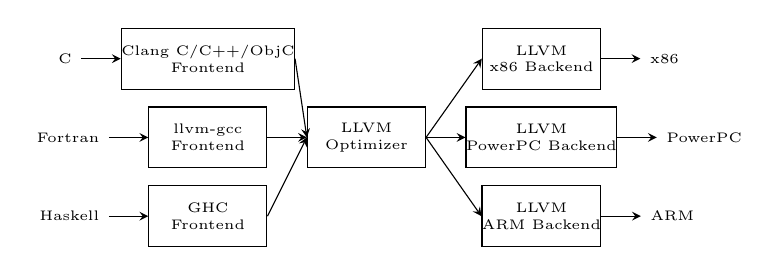
\begin{tikzpicture}[>=stealth]
    \tikzstyle{lang}=[rectangle,draw=black,thin,font=\tiny,inner
    sep=0pt, align=center,minimum width=1.5cm,minimum height=2.2em]

    \tikzstyle{txt}=[font=\tiny]

    \node[lang](llvm_opt){LLVM \\ Optimizer};
    \node[lang](ppc_back)[right=0.5 cm of llvm_opt]{LLVM \\ PowerPC Backend};
    \node[txt](ppc)[right=0.5 cm of ppc_back]{PowerPC};
    \node[lang](x86_back)[above of=ppc_back]{LLVM \\ x86 Backend};
    \node[txt](x86)[right=0.5 cm of x86_back]{x86};
    \node[lang](arm_back)[below of=ppc_back]{LLVM \\ ARM Backend};
    \node[txt](arm)[right=0.5 cm of arm_back]{ARM};

    \node[lang](gcc_front)[left=0.5 cm of llvm_opt]{llvm-gcc \\ Frontend};
    \node[txt](fortran)[left=0.5 cm of gcc_front]{Fortran};
    \node[lang](clang_front)[above of=gcc_front]{Clang C/C++/ObjC \\ Frontend};
    \node[txt](c)[left=0.5 cm of clang_front]{C};
    \node[lang](ghc_front)[below of=gcc_front]{GHC \\ Frontend};
    \node[txt](haskell)[left=0.5 cm of ghc_front]{Haskell};

    \draw[->] (clang_front.east) -- (llvm_opt.west);
    \draw[->] (gcc_front.east) -- (llvm_opt.west);
    \draw[->] (ghc_front.east) -- (llvm_opt.west);

    \draw[->] (llvm_opt.east) -- (x86_back.west);
    \draw[->] (llvm_opt.east) -- (ppc_back.west);
    \draw[->] (llvm_opt.east) -- (arm_back.west);

    \draw[->] (x86_back) -- (x86);
    \draw[->] (ppc_back) -- (ppc);
    \draw[->] (arm_back) -- (arm);

    \draw[->] (c) -- (clang_front);
    \draw[->] (fortran) -- (gcc_front);
    \draw[->] (haskell) -- (ghc_front);
  \end{tikzpicture}
  \caption{LLVM typical workflow \cite{llvm_general}}
  \label{fig:llvm_flow}
\end{figure}

\subsubsection{LLVM IR.}

The LLVM IR is the intermediate representation language of the LLVM
project. On its own it is a first-class language with well defined
semantics \cite{llvm_general,llvmmasterthesis}. Variables are in the SSA (Static Single
Assignment) form meaning that they can only be assigned once and they
keep that value for their entire lifetime. All the values residing in
memory need to be loaded to a variable first and stored back to memory
if they wish to be saved. Instructions operate solely upon
variables. In this respect, the LLVM IR resembles the assembly
language of an infinitely many registers Load-Store based RISC
processor.

The central concept in constructing LLVM IR is the Module. Each module
consists of functions, global variables and symbol table entries.
Modules can be combined using the LLVM linker \cite{llvm_ir}.

\subsection{GEZEL: A Hardware Description Language}
\label{gezel}

GEZEL\footnote{http://rijndael.ece.vt.edu/gezel2/} is a cycle-accurate hardware description language (HDL) using the
Finite-State-Machine + Datapath (FSMD) model. The basic element is a Signal Flow Graph (SFG). It groups operations that
are to be executed concurrently in the same clock cycle. One or more of these SFGs are used to form a datapath, which is the
main building block. A datapath is the smallest GEZEL unit that can stand on
its own and be simulated. Datapaths can be thought of as
\emph{modules} in Verilog or \emph{entities} in VHDL.

Figure \ref{fig:gezel_workflow} shows how the GEZEL language
can be used as an input to the following tools: \emph{fdlvhd}, a generator that can output synthesizeable VHDL or Verilog code; \emph{fdlsim}, a cycle accurate simulator used to verify and validate the design; and \emph{gplatform}, a co-simulation tool used for HW/SW co-design purposes.

\begin{figure}[hb!]
  \centering
  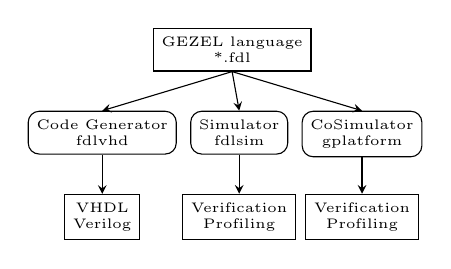
\begin{tikzpicture}[>=stealth, font=\tiny]
    \tikzstyle{edge from parent}=[draw,->]

    \Tree[.\node[language](fdl){GEZEL language \\ *.fdl};
      [.\node[compiler](fdlvhd){Code Generator \\ fdlvhd};
        [.\node[language](vhdl){VHDL \\ Verilog};]
      ]
      [.\node[compiler](fdlsim){Simulator \\ fdlsim};
        [.\node[language](sim){Verification \\ Profiling};]
      ]
      [.\node[compiler](gplatform){CoSimulator \\ gplatform};
        [.\node[language](cosim){Verification \\ Profiling};]
      ]
    ]
  \end{tikzpicture}
  \caption{GEZEL workflow}
  \label{fig:gezel_workflow}
\end{figure}

The co-simulation tool allows to cosimulate GEZEL designs with
instruction-set simulations. Supported processors include
ARM, AVR, 8051, MicroBlaze and PicoBlaze. The cosimulation tool allows
for designing a processor-coprocessor pair for a general purpose
processor and a custom dedicated coprocessor~\cite{Schaumont}.

%%% Local Variables:
%%% TeX-PDF-mode: t
%%% TeX-master: "paper"
%%% End:


\section{Custom Framework}
In this section we describe the main functionalities of our
framework. We first give an overview of our proposed solution, and
then we detail the concrete extensions we have performed on the PIL
language. The description of the PIL Front-End and the target
Back-Ends are also covered in this section.
\label{customframework}

\subsection{Framework Overview}
\label{frameworkoverview}
We propose a custom ZPKP compiler framework that takes a protocol
implementation in PIL as generated by the CACE ZKPK compiler and
produces GEZEL or C+GMP code. This allows exploring both ends of the
hardware-software co-design spectrum.
Figure~\ref{fig:custom_framework_workflow} gives an overview of the
custom framework.

\begin{figure}[hb!]
  \centering
  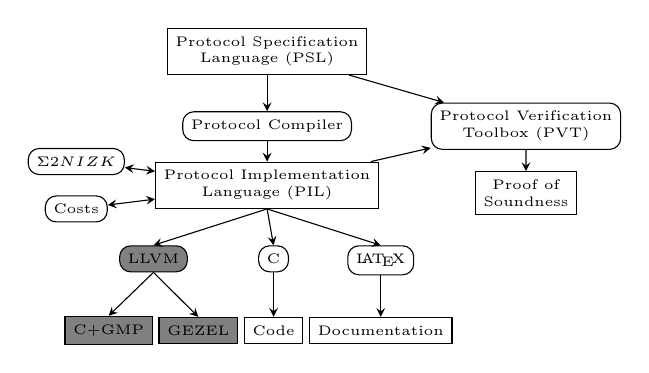
\begin{tikzpicture}[>=stealth,level distance=0.85cm, font=\tiny]
    \tikzstyle{edge from parent}=[draw,->] \tikzset{every leaf
      node/.style={anchor=center}}

    \Tree [.\node[language](psl){Protocol Specification \\ Language (PSL)};
      [.\node[compiler](pc){Protocol Compiler};
        [.\node[language](pil){Protocol Implementation \\ Language (PIL)};
          [.\node[compiler,added](llvm){LLVM};
            \node[language,added](asm){C+GMP};
            \node[language,added](gezel){GEZEL};
          ]
          [.\node[compiler](c){C}; \node[language](code){Code};]
          [.\node[compiler](latex){\LaTeX}; \node[language](doc){Documentation};]
        ]
      ]
    ]

    \node[compiler] (pvt)         [right=of pc,anchor=west]          {Protocol Verification \\ Toolbox (PVT)}
    child {node[language] {Proof of \\ Soundness}};

    \node[compiler] (sigma) [left=of pil.north west,anchor=center] {$\Sigma 2 N I Z K$};
    \node[compiler] (cost) [left=of pil.south west,anchor=center] {Costs};

    \draw[<->] (sigma) -- (pil);
    \draw[<->] (cost) -- (pil);

    \draw[->] (psl) -- (pvt);
    \draw[->] (pil) -- (pvt);
  \end{tikzpicture}
  \caption{Custom framework (extensions to CACE Zero Knowledge
    Compiler highlighted)}
  \label{fig:custom_framework_workflow}
\end{figure}

The generated code from the CACE ZKPK compiler is linked with a
supporting library that is not suitable for small-embedded
devices. The supporting library uses GMP but adds additional
complexity atop. Additionally, our extensions to PIL make it
incompatible with CACE ZKPK compiler.

In order to allow compatibility and improve performance we provide a
software back-end via GMP as well. In our case, there is no added
complexity or semantics. Additionally, we note that these basic GMP
semantics allow us to emulate a target supporting arbitrary-precision
arithmetic.

LLVM was chosen as the compiler framework to transform ZKPK
implementations in PIL into implementations in the desired
languages. The worfklow is depicted in Figure
\ref{fig:custom_llvm_workflow}. The starting point is a ZKPK
implementation in PIL which is compiled to LLVM IR code. The
implementation in LLVM IR can then be used as a starting point for
multiple targets. Section~\ref{targetbackends} describes the C+GMP and
GEZEL back-ends, along with some extensions to GEZEL. Extensions to
PIL are described in Section~\ref{extensionsPIL}.
\begin{figure}[hb!]
  \centering
  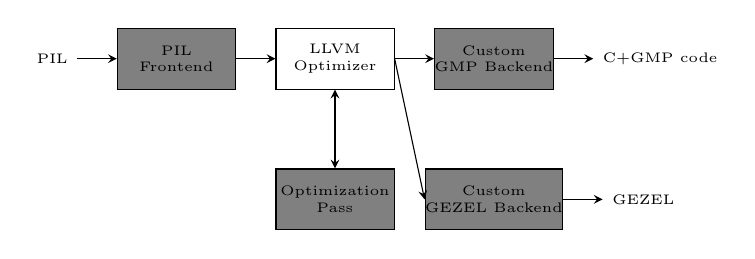
\begin{tikzpicture}[>=stealth]
    \tikzstyle{lang}=[rectangle,draw=black,thin,font=\tiny,inner
    sep=0pt, align=center,minimum width=1.5cm,minimum height=2.2em]

    \tikzstyle{txt}=[font=\tiny]

    \node[lang](llvm_opt){LLVM \\ Optimizer};

    \node[lang,added](gmp_back)[right=0.5 cm of llvm_opt]{Custom \\ GMP Backend};
    \node[txt](gmp)[right=0.5 cm of gmp_back]{C+GMP code};

    \node[lang,added](gezel_back)[below=of gmp_back]{Custom \\ GEZEL Backend};
    \node[txt](gezel)[right=0.5 cm of gezel_back]{GEZEL};

    \node[lang,added](llvm_pass)[below=1 cm of llvm_opt]{Optimization \\ Pass};

    \node[lang,added](pil_front)[left=0.5 cm of llvm_opt]{PIL \\ Frontend};
    \node[txt](pil)[left=0.5 cm of pil_front]{PIL};

    \draw[->] (pil_front.east) -- (llvm_opt.west);

    \draw[->] (pil) -- (pil_front);

    \draw[->] (llvm_opt.east) -- (gezel_back.west);
    \draw[->] (llvm_opt.east) -- (gmp_back.west);

    \draw[->] (gezel_back) -- (gezel);
    \draw[->] (gmp_back) -- (gmp);

    \draw[<->] (llvm_opt) -- (llvm_pass);
  \end{tikzpicture}
  \caption{LLVM custom workflow (changes highlighted)}
  \label{fig:custom_llvm_workflow}
\end{figure}


%\subsection{Extensions to CACE Zero-Knowledge Proofs Compiler}
%\label{extensions}

\subsection{Extensions to PIL}
\label{extensionsPIL}

\paragraph{Multiple Blocks.}
PIL specifies Prover and Verifier using respective blocks. A block can
comprise several functions, representing each of the protocol
rounds. The execution order of these rounds should also be
specified. Rounds are executed sequentially.

Besides Prover and Verifier, only an additional Common block, which
contains declarations visible to all the blocks, can be
specified. This makes it impossible to implement a multiparty
protocol, such as the DAA~\cite{DBLP:conf/ccs/BrickellCC04}. We allow
multiple blocks via a simple relaxation of the rules.

\paragraph{Global Variable Access.}
To assure the integrity of the variables in PIL, we have constrained
the language such that global variables can only be modified by the
executing round. This allows the global variable to be backed by a
local variable, which represents the value of the global variable for
the entire duration of the round. Only the last modification gets
written back to the global variable. This has the effect of converting
the CFG to a trivial one with a single node. Previously, the
instructions dominated by the value of the load instruction could not
be executed before the load instruction completed. Without the load
instruction, the ordering can again be arbitrary given the DFG is
satisfied.

The global variables are usually stored in a higher-latency, slower
access storage (register or cache or main memory) so this constraint
will actually improve the performance by accessing the global only
once per read or write.

By introducing this constraint we also protect the implementations
from side-channel attacks. The attacker cannot easily deduce the
location of the storage location of the global variable before the
global variable is actually read. Since the read and write need to
happen only once per round, the time available to launch an attack is
very short.

\paragraph{Compile Time/Constant Expressions.} PIL does not allow
constant expressions as parameters of variables. For example, the following code to declare an integer $f$ of length $l_f + l_{phi} + l_H$ is not allowed.
\begin{lstlisting}[language=PIL]
Common (
  Z l_f = 160;
  Z l_phi = 80;
  Z l_H = 160;
) {}
Smartcard (
  Int(l_f + l_phi + l_H) f
) {}
\end{lstlisting}
Without constant expressions, one would need to recompute the values
manually and re-enter them every time a modification is needed, which is prone to errors. Therefore, we provide PIL with this feature.

\paragraph{Type inference.}
Type inference allows to determine the resulting
type of a certain expression and can also be used to omit
a type declaration. The following example illustrates this:
\begin{lstlisting}[language=PIL]
Zmod*(p) b;
x := Random(Int(80));
a := b^x;
\end{lstlisting}
The type of x can be inferred as Int(80) since
the Random function can only return a random value of the provided
type. As for variable a, since the operation of exponentiation is defined as
applying the multiplication operation many times, the type is Zmod*(p). A similar argument holds when multiplying an element
of the additive modular residue group with an integer. Consequently,
type inference is well defined for any acceptable operation in PIL.

\subsection{Target Back-ends}
\label{targetbackends}
\paragraph{Extensions to GEZEL.}
\label{extensionsGEZEL}

In order to implement modular arithmetic in GEZEL, it is necessary to
follow a two step approach. First, the operation is executed over the
integers, and, second, the modular reduction of the result is
calculated. This approach is valid to implement addition, subtraction
and multiplication, but it cannot be used to support modular
exponentiations.

There are two methods to solve this lack of support: either simulate a
modular exponentiation via implementing it in GEZEL, or extend GEZEL
so that it provides support for modular exponentiation. The latter
approach was taken since it was deemed necessary to enrich the
language with this operation.

\paragraph{GEZEL Back-end.}
\label{gezelbackend}
The GEZEL back-end designs a purely hardware, purely intra-round
combinatorial design. Our PIL semantics allow global variables to be
read at most once and written at most once without any imposed
order. Since there is no enforced order, this allows us to schedule
all the operations in a single clock-cycle.

\paragraph{GMP Back-end.}
\label{gmpbackend}
All of the architectures LLVM supports lack multi-precision arithmetic
support.  This multi-precision support has to come from the software
side via a support library. GMP was chosen as it was deemed the best
option given stability, licensing and performance. The performance
results are due to the efficiency of the GMP library. In this manner,
we take after the CACE ZKPK Compiler.

%%% Local Variables:
%%% TeX-PDF-mode: t
%%% TeX-master: "paper"
%%% End:


\section{Discussion}
\label{discussion}

\subsection{Optimizations}

LLVM provides a constant folder which allows constant expressions to
be evaluated at compile time. This eliminates all the redundant calls
that would otherwise be needed at run-time, which can reduce the number
of complex, costly arbitrary-precision operations.

LLVM IR is of the static single assignment form, which allows
aggressive optimizations such as dead-code elimination. Another
advantage of LLVM is the possibility of separating the optimizations
to higher level (common back-end) and lower level (specific back-end).

\paragraph{Common Back-end Optimizations.}
In the following we describe optimizations that are valid for all the
back-ends since they are abstract enough to be applicable without
knowing the back-end specifics.

Since accessing the global variables is slower, writing to the global
variable can be left for the end of the current round or deferred to a
later time, when needed. This allows optimizations in a
hardware-software co-design world where it can be expensive to move
data around.  The optimization is achieved by traversing all the load
instructions that follow a store instruction.  If any of those load
instructions loads from the same location which a store location wrote
to, all the nodes that are dominated by the loaded value are replaced
with the value that was stored. In our model of computation this is
perfectly sane since only the current round can modify a global
variable.

Another optimization example we can think of is exponentiation via
Montgomery multiplications. If we were to translate all the operations
of the algorithm step-by-step, we would have a transfer to the
Montgomery domain, multiplication in the Montgomery domain and return
from the Montgomery domain. The high-level optimizer can eliminate the
unnecessary transfers and returns since they are inverse operations
performed consecutively.

\paragraph{Specific Back-end Optimizations.}
GMP supports a function that integrates multiplication and addition.
When the result of a multiplication is used only in the addition
following it, the back-end can replace both operations with a single
invocation to the supporting GMP function.

GMP has a lower-level set of functions which are used to implement all
the other functions within the GMP library. These functions are more
efficient at the expense of generality and coherence of the interface.
The LLVM IR could be directly transformed to these lower-level
functions to gain efficiency.

Another possibility consists in using a different arbitrary-precision
library, such as CLN\footnote{http://www.ginac.de/CLN/},
OpenSSL\footnote{http://www.openssl.org} or
libgcrypt\footnote{http://directory.fsf.org/project/libgcrypt/}. CLN
offers group types and modular arithmetic and it would have been a
better choice were it not for the loss of information by using integer
types to represent group types in the LLVM IR. Additionally, the GMP
library offers a possibility of reusing a faster modular
multiplication algorithm than the Montgomery algorithm~\cite{Montgomery85}.

\subsection{Security Analysis}

CACE ZKPK Compiler already offers a formal proof of correctness
covering the transformation from PSL to PIL. We need to analyze the
security of the transformation from PIL to LLVM IR and LLVM IR to the
back-ends whenever possible.

LLVM IR allows us to verify the correctness of the types since LLVM IR
uses code of the static single assignment form, where every variable
is assigned a value exactly once. This allows security assertions to
be taken to a lower level than the one allowed by CACE. 

To assure the correctness of types, first it is necessary to lay out
the DFG of the protocol round. For each node of the DFG preconditions
and postconditions cab be established, such as the ones in Table
\ref{tab:basic_nodes}. Hoare logic~\cite{hoare_logic} can then be
used to prove the correctness of the transformation from PIL to the
LLVM IR.

As for the transformation of LLVM IR into target implementations, it
might not always be possible to prove correctness, especially if the
target implementation is hardware. Since it is impossible to make this
assurance it was deemed unnecessary to go this low and the blocks are
assumed to be correct (if the preconditions are satisfied, the
postconditions will be assured by the block). For the software case,
such properties are assured by the library used.

\begin{table}[h!]
  \centering
  \begin{tabular}{l | c | c}
    Basic block        & Preconditions             & Postconditions \\
    \hline
    Modular adder      & $x \in Z_q^+, y \in Z_q^+$ & $z \in Z_q^+$ \\ 
    Modular multiplier & $x \in Z_p^*, y \in Z_p^*$ & $z \in Z_p^*$ \\
    Zero extender      & $x \in Z_p$               & $z \in Z_p$
  \end{tabular}
  \caption{Basic Nodes}
  \label{tab:basic_nodes}
\end{table}

%%% Local Variables: 
%%% TeX-PDF-mode: t
%%% TeX-master: "main"
%%% End: 


\section{Use Case: Schnorr's Protocol}
\label{schnorr}

The Schnorr's Identification Protocol is a simple
$\Sigma$-protocol. Here we demonstrate how our extensions do not
disrupt the CACE Project ZKC flow but merely complement it. An input
PSL file is given to the CACE Project ZKC and a corresponding PIL file
is received. This PIL file is processed using our framework to
generate both a GEZEL and a GMP target. These are then cross-validated
with the C code that the CACE Project ZKC generates. This was made
possible thanks to the implemented terminal port communication
library.

\subsection{A custom co-processor system}

We took a step further into demonstrating hardware-software co-design
using our framework and have wrote a back-end for an existing
co-processor system. The main processor of this system is an 8051 as
is commonly found on most
smart-cards~\cite{smartcard_crypto_coprocs2}. The 8051 is a very
limited processor and a custom co-processor is needed if cryptography
applications are to be targeted. This leads to a trade-off in terms of
execution time and size as the more operations are implemented in the
co-processor the execution time is lower but the size required is
larger. The project deemed the Montgomery multiplication the most
critical and has implemented it as the only operation on the
co-processor.

The back-end's job was merely to reuse the existing libraries provided
by the co-processor designers but we still believe it was sufficient
to show the feasibility of the approach of this framework. The
execution time was around $2,000,000$ cycles which on a
$\unit[4]{MHz}$ system (common frequency as mentioned in
\cite{smartcard_crypto_coprocs2}) is roughly $\unit[0.5]{s}$.

%%% Local Variables: 
%%% TeX-PDF-mode: t
%%% TeX-master: "paper"
%%% End:


\section{Conclusion and Future Work}
\label{conclusion}
\chapter{Conclusion}

%%% Local Variables: 
%%% TeX-PDF-mode: t
%%% TeX-master: "thesis"
%%% End: 


\bibliographystyle{IEEEtran}
\bibliography{main}

\end{document}

%%% Local Variables: 
%%% TeX-PDF-mode: t
%%% TeX-master: t
%%% End: 
